%=== CHAPTER ONE (1) ===
%=== INTRODUCTION ===

\chapter{Introduction}

\section{Background}

SLAM(Simultaneous localization and mapping) is a key component in mobile autonomous systems. It describes the ability of a vehicle, once placed in an unknown environment, to explore and map that environment, while at the same time estimating its own position in the environment, using only its onboard sensing capabilities.

SLAM systems can be accomplished by both single or multiple robots. Multiple-robot SLAM or MRSLAM, offer several advantages compared to there single robot counterpart, for example:
\begin{itemize}
	\item Robustness to single robot failure,
	\item Quicker exploration of environments in time critical SaR(Search and Rescue) mission.
\end{itemize} 


However, Adapting SLAM technology to multiple-robot scenario brings some new changes as identified by Saeedi et al \cite{saeedi2016multiple}:
\begin{itemize}
	\item Relative Poses of Robots. In multiple-robot SLAM, the map provided by each robot in its own reference coordinates is called the local map. It is difficult task to integrate all of the local maps provided by the other robots to generate a global map of the environment, because the required alignments or transformation matrices, which relate these maps to each other, are in general unknown.
	\item Closing Loops. Loop closure, is defined as identifying a place observed previously but not very recent. Solving this problem for a team of multiple robots requires using all resources of information from individual robots.in Multi-robot SLAM, various events can trigger loop closure, such as direct encounter of the robots or rendezvous and indirect encounter, when the robots see the same area of features in the world.
	\item Communications. Availability of a medium for data sharing among robots is an important requirement in multiple‐robot SLAM. Information between robots can be exchanged via communication channels. The quality of the communication channels is dependent on the environment. For instance, communication issues are a challenging problem for a team of robots in underwater environments, where the environment imposes limitations on the bandwidth and data rate.
\end{itemize}

Because of the limitation of the difficulties mentioned above, the development of multiple-robot SLAM is much slower than single-robot SLAM. Finding a solution to these problem will push the adaption of SLAM technology to a new level.

\begin{figure}[H]
\centering
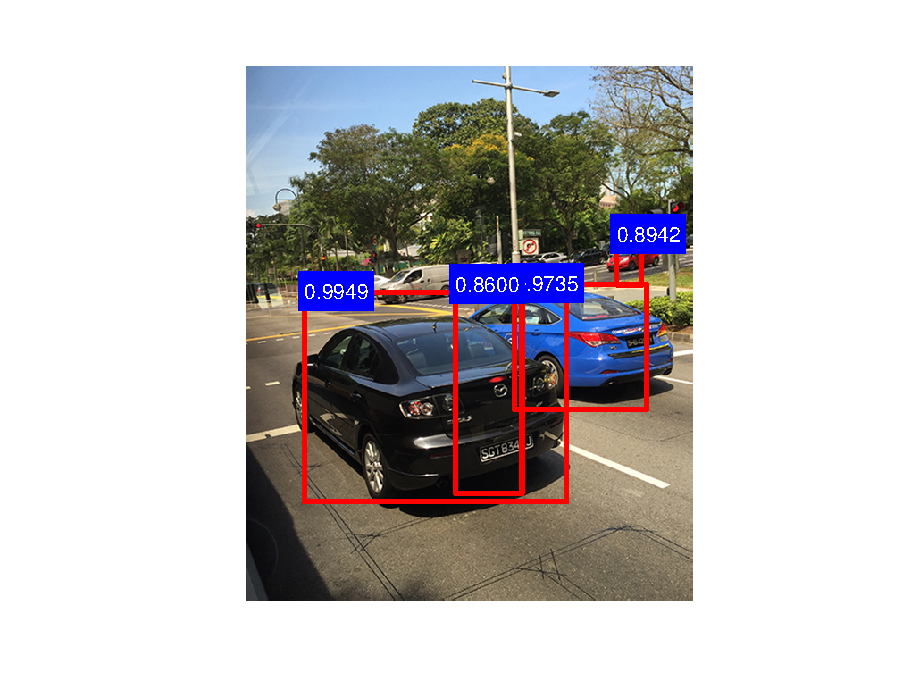
\includegraphics[width=4in]{Chapter1/boundingbox.eps}
\caption{TBD}
\label{fig:boundingboxexample} 
\end{figure}


\section{Motivation and Objectives}

Recently, some solutions for Multi-robot SLAM systems have been proposed.\cite{mcmanus2014shady}




\section{Major contribution of the Dissertation}
\begin{enumerate}[1.]
	\item Evaluation of CORB-SLAM on NTU datasets collected by a cluster of multi ground robots or multi hybrid robots.
	\item Modification of CORB-SLAM to improve its stability and accuracy.
	\item Combination of CORB-SLAM and shade dealing algorithms to enhance its ability to deal with illumination changes.
\end{enumerate}


\section{Organisation of the Dissertation}
This dissertation is organised into several chapters:
\begin{enumerate}[1.]
	\item Chapter 2 briefly outlines the development of visual SLAM technique. Firstly, the classic structure of visual SLAM system is introduced, and the critical algorithms involved are elaborated. The existing solutions are classified into single-robot and multi-robot systems. This chapter also explores prior work in shade dealing algorithms required to implement life-long SLAM.
	
	\item Chapter 3 explains the methodology used in this dissertation to improve the stability and accuracy of CORB-SLAM, and how to combine illumination variance method with CORB-SLAM system to enhance the ability of CORB-SLAM to deal with illumination changes.
	
	\item Chapter 4 shows the results of 
	\begin{inparaenum}[(i)]
		\item the evaluation of CORB-SLAM with NTU datasets.
		\item the evaluation of illumination variant CORB-SLAM with datasets collected under different illumination conditions.
		\end{inparaenum}
		
	\item Chapter 5 analysis the results demonstrated in chapter 4 in detail, discussing the improvement and the disadvantages.
	
	\item Chapter 6 summarizes the work done in this dissertation, and comments on the significance and some potential applications of the proposed solutions.  

\end{enumerate}


%=== END OF CHAPTER ONE ===
\newpage


